\documentclass[11pt]{article}
 
\usepackage[text={6in,8.1in},centering]{geometry}
 
\usepackage{enumerate}
\usepackage{amsmath,amsthm,amssymb}
 
\usepackage{pstricks}
\usepackage{pst-solides3d}
\usepackage{pstricks-add}
\usepackage{graphicx}
\usepackage{pst-tree}
\usepackage{pst-poly}
\usepackage{calc,ifthen}
\usepackage{float}
\usepackage{multicol}
\usepackage{multirow}
\usepackage{array}
\usepackage{longtable}
\usepackage{tikz}
\usepackage{tkz-berge}
\usepackage{fancyhdr}
\usepackage{algorithmicx}
\usepackage{algpseudocode}
\usepackage{changepage}

\newenvironment{block}{\begin{adjustwidth}{1.3cm}{1.3cm}\noindent}{\end{adjustwidth}}

\newtheorem{proposition}{Proposition}
\newtheorem{theorem}{Theorem}
\newtheorem{lemma}{Lemma}
\newtheorem{corollary}{Corollary}
 
\theoremstyle{definition}
\newtheorem{definition}{Definition}
 
\title{Cayley Digraphs of Finite Cyclic Groups with Minimal Diameter\footnote{Supported in part by National Science Foundation (NSF).}}
\author{Jordan Blocher\thanks{Department of Mathematics, University of Nevada-Reno, Reno, NA, USA. jordanblocher@gmail.com.}\and Christopher Linden\thanks{University of California Los Angeles, Los Angeles, CA,USA } \and Samantha Hampton\thanks{Department of Mathematics, University of Arkansas, Fayetteville, AR, USA}}
\date{\today}
 
 
\def\R{\mbox{$\mathbb R$}}
\def\Q{\mbox{$\mathbb Q$}}
\def\Z{\mbox{$\mathbb Z$}}
\def\N{\mbox{$\mathbb N$}}
\def\C{\mbox{$\mathbb C$}}
\def\Sym{\operatorname{Sym}}
\def\lcm{\operatorname{lcm}}
\def\adj{\operatorname{adj}}
\def\inc{\operatorname{inc}}
\def\Cay{\operatorname{Cay}}
\def\Geom{\operatorname{\cal G}}
\def\ker{\operatorname{ker}}
\def\kernel{\operatorname{ker}}
\def\automorphism{\operatorname{Aut}}
\def\endomorphism{\operatorname{End}}
\def\inner{\operatorname{Inn}}
\def\outer{\operatorname{Out}}
\def\crossing{\operatorname{cr}}
\def\cent{\textcent}
\def\n{\\ \vspace{1.7mm}}
 
\renewcommand{\emptyset}{\O}
 
 
\newcounter{ZZZ}
\newcounter{XXX}
\newcounter{XX}
 
\headsep25pt\headheight20pt
 
 
\pagestyle{fancyplain}
\lhead{\fancyplain{}{\small\bfseries Authors,\ \ This is our Title}}
\rhead{\fancyplain{}{\small\bfseries\thepage}}
\cfoot{\ \hfill\tiny\sl Draft printed on \today}
 
 
\setlength{\extrarowheight}{2.5pt} % defines the extra space in tables
 
 
 
\begin{document}
 
\maketitle
\begin{center}
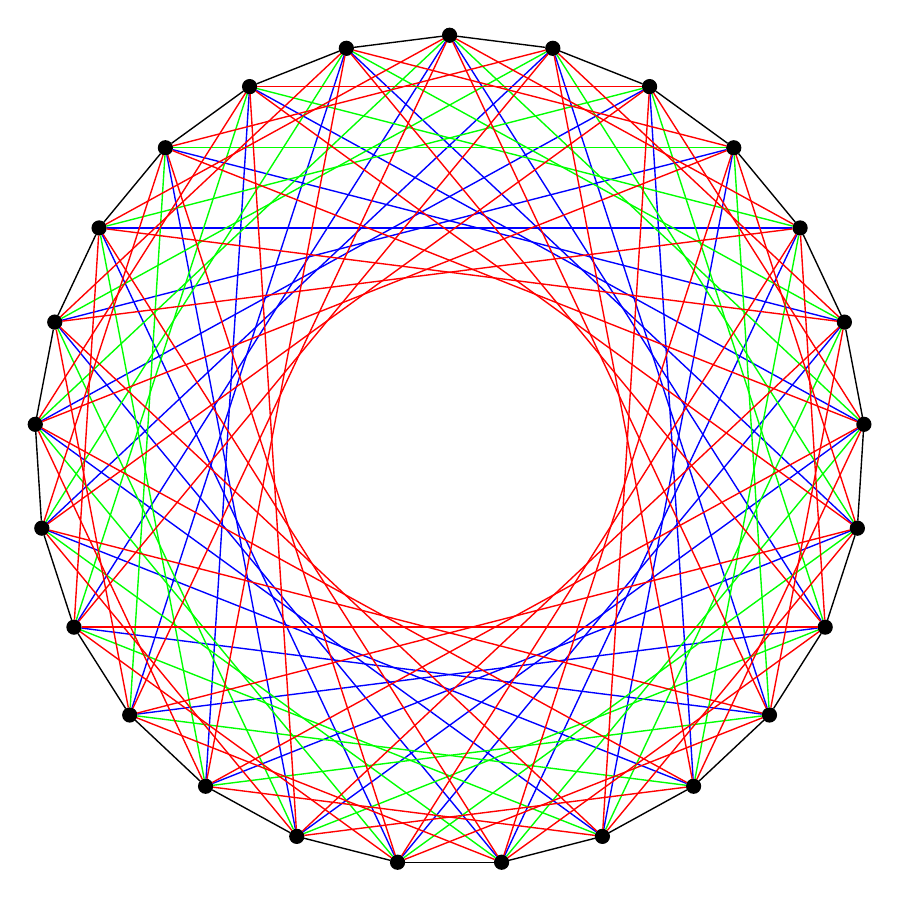
\begin{tikzpicture}


\GraphInit[vstyle=Simple]
\tikzset{VertexStyle/.append style = {minimum size = 5pt, inner sep = 0pt}}

\Vertex[x=187.5pt,y=337.5pt]{0};
\Vertex[x=224.80348307472823pt,y=332.7874741692947pt]{1};
\Vertex[x=259.7630511152573pt,y=318.94600200657953pt]{2};
\Vertex[x=290.1820658893033pt,y=296.8452941132117pt]{3};
\Vertex[x=314.14918882530225pt,y=267.87401924684946pt]{4};
\Vertex[x=330.15847744427305pt,y=233.85254915624213pt]{5};
\Vertex[x=337.2040092642407pt,y=196.91857792939703pt]{6};
\Vertex[x=334.8430876093033pt,y=159.3928028121413pt]{7};
\Vertex[x=323.22405786990294pt,y=123.63310626523908pt]{8};
\Vertex[x=303.0769864163684pt,y=91.88640153769651pt]{9};
\Vertex[x=275.667787843871pt,y=66.14745084375791pt]{10};
\Vertex[x=242.71868290270174pt,y=48.0335271167623pt]{11};
\Vertex[x=206.2999850346457pt,y=38.682794802828326pt]{12};
\Vertex[x=168.70001496535434pt,y=38.682794802828326pt]{13};
\Vertex[x=132.2813170972983pt,y=48.03352711676226pt]{14};
\Vertex[x=99.3322121561291pt,y=66.14745084375782pt]{15};
\Vertex[x=71.92301358363159pt,y=91.88640153769656pt]{16};
\Vertex[x=51.77594213009703pt,y=123.63310626523916pt]{17};
\Vertex[x=40.1569123906967pt,y=159.3928028121413pt]{18};
\Vertex[x=37.795990735759275pt,y=196.91857792939695pt]{19};
\Vertex[x=44.841522555726954pt,y=233.8525491562421pt]{20};
\Vertex[x=60.85081117469775pt,y=267.8740192468495pt]{21};
\Vertex[x=84.81793411069665pt,y=296.8452941132117pt]{22};
\Vertex[x=115.23694888474257pt,y=318.9460020065795pt]{23};
\Vertex[x=150.1965169252717pt,y=332.7874741692946pt]{24};

\SetUpEdge[lw         = .5pt,
            color      = black,
            labelcolor = black]

\Edge(24)(0)
\Edge(0)(1)
\Edge(1)(2)
\Edge(2)(3)
\Edge(3)(4)
\Edge(4)(5)
\Edge(5)(6)
\Edge(6)(7)
\Edge(7)(8)
\Edge(8)(9)
\Edge(9)(10)
\Edge(10)(11)
\Edge(11)(12)
\Edge(12)(13)
\Edge(13)(14)
\Edge(14)(15)
\Edge(15)(16)
\Edge(16)(17)
\Edge(17)(18)
\Edge(18)(19)
\Edge(19)(20)
\Edge(20)(21)
\Edge(21)(22)
\Edge(22)(23)
\Edge(23)(24)

\SetUpEdge[lw         = .5pt,
            color      = blue,
            labelcolor = black]

\Edge(0)(8)
\Edge(2)(10)
\Edge(4)(12)
\Edge(6)(14)
\Edge(8)(16)
\Edge(10)(18)
\Edge(12)(20)
\Edge(14)(22)
\Edge(16)(24)
\Edge(18)(1)
\Edge(20)(3)
\Edge(22)(5)
\Edge(24)(7)
\Edge(1)(9)
\Edge(3)(11)
\Edge(5)(13)
\Edge(7)(15)
\Edge(9)(17)
\Edge(11)(19)
\Edge(13)(21)
\Edge(15)(23)
\Edge(17)(0)
\Edge(19)(2)
\Edge(21)(4)
\Edge(23)(6)

\SetUpEdge[lw         = .5pt,
            color      = green,
            labelcolor = black]

\Edge(0)(6)
\Edge(6)(12)
\Edge(12)(18)
\Edge(18)(24)
\Edge(24)(5)
\Edge(5)(11)
\Edge(11)(17)
\Edge(17)(23)
\Edge(23)(4)
\Edge(4)(10)
\Edge(10)(16)
\Edge(16)(22)
\Edge(22)(3)
\Edge(3)(9)
\Edge(9)(15)
\Edge(15)(21)
\Edge(21)(2)
\Edge(2)(8)
\Edge(8)(14)
\Edge(14)(20)
\Edge(20)(1)
\Edge(1)(7)
\Edge(7)(13)
\Edge(13)(19)
\Edge(19)(0)

\SetUpEdge[lw         = .5pt,
            color      = red,
            labelcolor = black]

\Edge(0)(4)
\Edge(4)(8)
\Edge(8)(12)
\Edge(12)(16)
\Edge(16)(20)
\Edge(20)(24)
\Edge(24)(3)
\Edge(3)(7)
\Edge(7)(11)
\Edge(11)(15)
\Edge(15)(19)
\Edge(19)(23)
\Edge(23)(2)
\Edge(2)(6)
\Edge(6)(10)
\Edge(10)(14)
\Edge(14)(18)
\Edge(18)(22)
\Edge(22)(1)
\Edge(1)(5)
\Edge(5)(9)
\Edge(9)(13)
\Edge(13)(17)
\Edge(17)(21)
\Edge(21)(0)
\Edge(0)(9)
\Edge(9)(18)
\Edge(18)(2)
\Edge(2)(11)
\Edge(11)(20)
\Edge(20)(4)
\Edge(4)(13)
\Edge(13)(22)
\Edge(22)(6)
\Edge(6)(15)
\Edge(15)(24)
\Edge(24)(8)
\Edge(8)(17)
\Edge(17)(1)
\Edge(1)(10)
\Edge(10)(19)
\Edge(19)(3)
\Edge(3)(12)
\Edge(12)(21)
\Edge(21)(5)
\Edge(5)(14)
\Edge(14)(23)
\Edge(23)(7)
\Edge(7)(16)
\Edge(16)(0)

\end{tikzpicture}
\end{center}
 
$\\$
$\\$
$\\$

\begin{abstract}
For positive integers $d$ and $k$ let $m(d,k)$ be defined to be the maximum modulus m such that there exists a generating set A of the \emph{Cayley digraph} Cay(m, A) with cardinality equal to k such that the diameter of Cay(m, A) is less than or equal to d. 
\end{abstract}
 
\section{Introduction}
 
Let $\Gamma$ be a finite group with a subset A. The \emph{Cayley digraph}, denoted Cay($\Gamma$,A), is a digraph with vertex set $\Gamma$, such that (x,y) is a directed edge if and only if $yx^{-1}$ $\in$ A.
In this paper we will be working with $\mathbb{Z}_m$ as our vertex set, and will denote these Cayley graphs as Cay(m,A).
 

 \begin{figure}[h]
\begin{center}

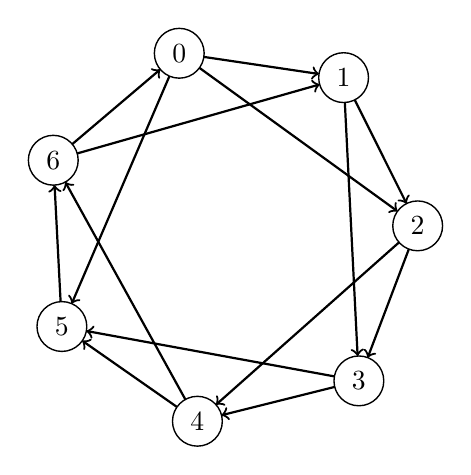
\begin{tikzpicture}


\Vertex[x=170.0508492385226pt,y=257.44793707070056pt]{0};
\Vertex[x=229.43059777036808pt,y=248.64351388167475pt]{1};
\Vertex[x=256.19943380501326pt,y=195.0860839875888pt]{2};
\Vertex[x=234.95343715746685pt,y=139.06822600729095pt]{3};
\Vertex[x=176.6059109911555pt,y=124.48269654626677pt]{4};
\Vertex[x=127.63862734371301pt,y=158.71121570275264pt]{5};
\Vertex[x=124.5266485799639pt,y=218.79228696858095pt]{6};
\tikzset{EdgeStyle/.style={->}}
\Edge(1)(2)
\Edge(0)(1)
\Edge(6)(0)
\Edge(5)(6)
\Edge(4)(5)
\Edge(3)(4)
\Edge(2)(3)
\Edge(0)(2)
\Edge(2)(4)
\Edge(4)(6)
\Edge(6)(1)
\Edge(1)(3)
\Edge(3)(5)
\Edge(0)(5)
\end{tikzpicture}
\end{center}
\caption{ Cay($\mathbb{Z}_7$, \{1,2\}).}
\end{figure}
 
An important property of Cayley digraphs is the Cayley digraph Cay(m,A) is vertex-symmetric. This property allows us to define extremal functions for these digraphs. 
For any positive integer $d$ we define
\[
m(d,A) =\ max\{m | diam(Cay(m,A)) \leq d\},
\]
the largest positive integer $m$ such that the diameter, d(m,A), of the Cayley digraph Cay(m,A) is less than or equal to d. For positive integers $d$ and $k$,
\[
m(d,k) = max\{m(d,A) | \text{ there exists a set A with } |A| = k \},
\]
the maximum modulus m such that there exists a generating set with cardinality equal to k and the diameter of the Cayley digraph is less than or equal to d. 
$\\$

Current known bounds include
\begin{align*}
m(1,k)& = k+1,\\
m(d,1) &= d+1\text{, and}\\
m(d,2) &=\left \lfloor \frac{d(d+4)}{3}\right \rfloor+1 \text{ for all } d\geq2.
\end{align*}
 
We will begin by examine the case when k = 3. The current bounds for this case, as $d\to\infty$, are
\[
\frac{176}{2197}d^3 + O(d^2) \leq m(d,3) \leq \frac{1}{14-3\sqrt{3}}(d+3)^3 .
\]
 



\section{The Algorithm}

We now provide an algorithm that takes as an input a set of generators as well as two other permutation sets. These inputs are used to test the ability of a generated lower bound to provide a set covering for our Cayley Graph. The algorithm iterates through permutations of the generating set and possible coverings, giving as an output the maximal generating set as well as the optimal polynomial bound.\\

Let $d$ be the diameter for $\Cay(m, k)$.\\

Given $d$ define $d_{1}$ fixed to be $\frac{d}{\lambda}$, also define $a_{1} = \frac{a}{\lambda}$, $b_{1} = \frac{b}{\lambda}$, and $c_{1} = \frac{c}{\lambda b}$, etc.., so $\lambda$ is a large number determined by $d$. The parameter $\lambda$ will not appear in the code, but it enables us to compute a lower bound as a function of $d$.\\

Our lower bound on $m(d, k)$ will be defined as $m =\alpha \lambda a_{1} + \beta \lambda b_{1} + \gamma \lambda c_{1}$+ ... $\psi \lambda z_{1}$.  To determine the validity of the lower bound, we compute every point in $dA$ as a polynomial in terms of $\lambda$.\\

$\forall$ ($x_{1}, x_{2}, ... , x_{n}$) such that $x_{1} \leq b_{1}, x_{2} \leq c_{1}, .. , x_{n} \leq \psi$ and $\sum_{i} x_{i} \leq d$ define polynomials that are considered to be (new term needed here).\\

$\forall$ constructed lower bounds $x = x_{1}a + x_{2}b + .. + x_{n}k$, we remove dependent linear combinations by comparing the coefficients $(x_{1}, x_{2}, x_{3}, .. , x_{n})$ and $(\alpha, \beta, \gamma, .. , \psi)$ from their respective polynomials.\\

The constructed lower bounds are defined to be regular if $x \in \mathbb{Z}_{m}$. In this way we are able to check $dA \cong to \mathbb{ZZ}_{m}$ by only considering a single representative of $\mathbb{Z}_{m}$.
\\ Note that a regular polynomial need not be minimal.\\

$\forall x \in dA$ if $x \notin Z_m$, we can identify $x$ with point $x' = (x'_{1}, x'_{2}, .. , x'_{k}) \in \mathbb{Z}_{m}$ congruent to $x$ $(mod$ $m)$.  Then if every point $n \in \mathbb{Z}_{m}$ is either equal to some $x$ or $x'$, $dA = \mathbb{Z}_m$. \\

Consider the case, $x > m(d, k)$, where $x$ is not regular. We perform a recursive polynomial subtraction of the coefficients where $\alpha, \beta, \gamma, ... , \psi$ is subtracted term-by-term from $x_{1}, x{2}, x{3}, ... , x{n}$. The resulting low-order coefficients are then forced to be positive by adding the generator associated with the next higher-order term.\\

For example, a resulting polynomial that has been forced to be well formed may look as, $[\lambda(x_{1} - 2 \alpha) + 1]a_{1} + [\lambda(x_{2} - 2 \beta) + 2]b_{1} + [\lambda(x_{3} - 2 \gamma]c_{1} + ... + [\lambda(x_{n} - 2 \psi]z_{1}]$.\\

To construct a lower bound, we systematically check combinations of generators $A$ and coefficients, and record the largest $m$ (and corresponding generators) such that a covering by $dA$ is achieved.

\subsection{Pseudocode}

\begin{algorithmic}

\ForAll{$X = (ax_{1} + bx_{2} + cx_{3} + .. + zx_{n}), M = (\alpha a + \beta b + \gamma c + .. + \psi z)$}  
\State X - M
\EndFor
\end{algorithmic}

\end {document}
